\section{Descriptive Analysis of the Dataset}
\label{sec:data-description}
This section updates the study's earlier data-description protocol to reflect the corpus actually used for the reported experiments. The study originally considered de-identified administrative archives, subject to access approvals, and supplemental simulated examples. Those were possible acquisition pathways, not completed observations. The experimental data currently consist entirely of \emph{researcher-constructed synthetic complaint narratives}; no authentic barangay records are presented as training data. The objective of using controlled synthetic text is to build an auditable and systematically varied classification benchmark, not to estimate how frequently a complaint type occurs in Davao City. Following Chicco et al.~\cite{chicco2022} and Bender and Friedman~\cite{benderfriedman}, the data's provenance, sampling choices, missing coverage and preprocessing choices are reported alongside model scores.

\subsection{Data Sources, Construction and Composition}
Source acquisition in this study refers to researching the \emph{foundations of scenario design}: Philippine barangay governance and topic-specific laws, administrative reporting guidance, studies of Filipino complaint speech acts and code-switching, and published approaches to spam and synthetic-text validation. Each of 60 Valid topics, 28 Suspicious review reasons and 30 Spam forms is tracked in the accompanying source-to-category matrix. These references provide topic or linguistic justification; they neither certify individual generated incidents as real nor imply the 118 categories are official government labels. Generation was carried out from researcher-designed incident descriptions and style frames; the existing fixed corpus is not being regenerated in this revision.

The corpus contains \textbf{24,000} records and \textbf{21 recorded fields}. Of those, the predictive input is \texttt{complaint\_text} and the target is \texttt{classification}. Supporting columns record category, language assignment, scenario or template family, provenance, assigned partition, and review-status flags. The raw unmodified CSV remains preserved within the research repository. All 24,000 source-type entries are marked \texttt{synthetic\_researcher\_constructed\_unreviewed}. This label distinguishes the corpus from real archived reports and from independently annotated gold-standard data.

\begin{table}[H]\centering\caption{Observed corpus composition and provenance}\label{tab:m1composition}\small
\begin{tabularx}{\textwidth}{p{0.42\textwidth}rX}\toprule
\textbf{Dimension} & \textbf{Records} & \textbf{Interpretation}\\\midrule
Entire research corpus & 24,000 & 100\% researcher-generated synthetic text\\
Valid & 8,000 & 33.33\% of corpus\\
Suspicious & 8,000 & 33.33\% of corpus\\
Spam & 8,000 & 33.33\% of corpus\\
Bisaya/Cebuano (assigned) & 6,000 & 25\% of corpus\\
Filipino (assigned) & 6,000 & 25\% of corpus\\
English (assigned) & 6,000 & 25\% of corpus\\
Mixed/code-switched (assigned) & 6,000 & 25\% of corpus\\
Verified human annotations & 0 & No independent label review recorded\\
Authentic archived complaints & 0 & Not a sampled administrative archive\\\bottomrule
\end{tabularx}\end{table}

\subsection{Exploratory Data Analysis and Text Characteristics}
Exploratory Data Analysis (EDA) was computed on the existing unprocessed \texttt{complaint\_text} values using whitespace-delimited word counts, class totals, assigned language totals and duplicate checks. Token length in this table is a reproducible whitespace-word count, not a universal measure of syllables or morphologically segmented Cebuano vocabulary. The corpus has no missing complaint narrative and no exact duplicate strings, but neither condition rules out meaning-equivalent paraphrases, repeated phrasal openings or near-duplicate source patterns.
\begin{table}[H]\centering\caption{Measured narrative lengths by supervisory label}\label{tab:m1lengths}\small\begin{tabular}{lrrrrr}\toprule
\textbf{Label} & \textbf{$n$} & \textbf{Mean} & \textbf{Median} & \textbf{Minimum} & \textbf{Maximum}\\\midrule
Valid & 8,000 & 20.76 & 20 & 5 & 48\\
Suspicious & 8,000 & 29.78 & 28 & 8 & 66\\
Spam & 8,000 & 14.90 & 15 & 1 & 35\\\bottomrule
\end{tabular}\end{table}
The overall corpus has a mean length of 21.81 words, median of 21 words, and observed range of 1--66 words. Figure~\ref{fig:m1lengths} displays the unequal within-class distributions. Suspicious entries average substantially longer than Spam, showing that an initially balanced class design can still encode unintended class cues in narrative length. This motivates the length-only and character-ngram diagnostics reported in Chapter~4; equal class totals alone cannot prevent superficial shortcuts.
\begin{figure}[H]\centering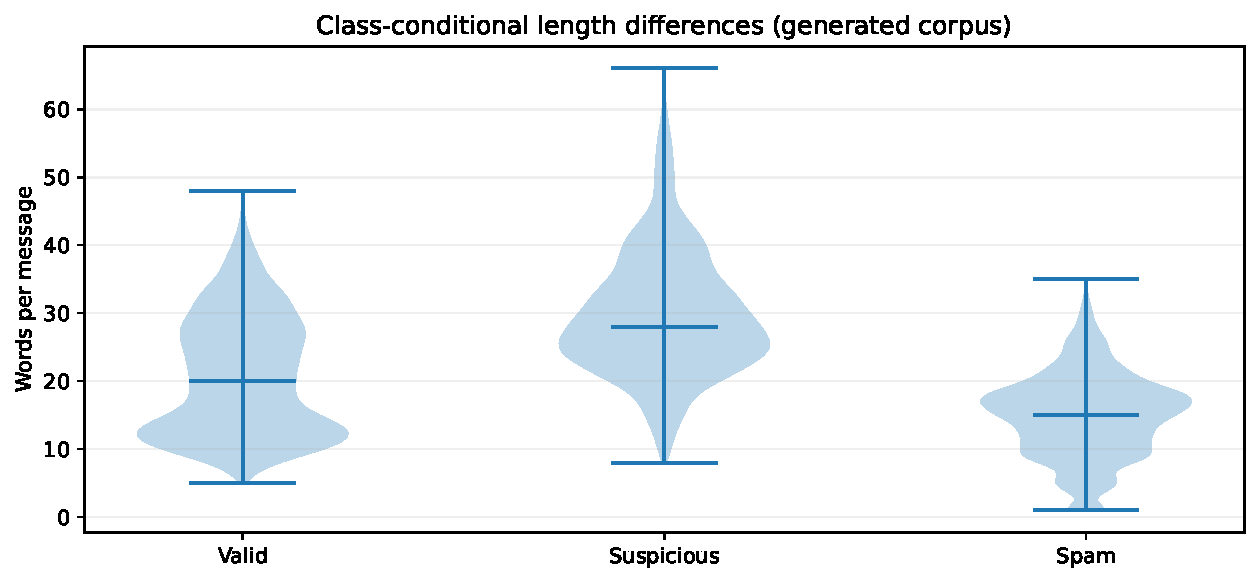
\includegraphics[width=.86\textwidth]{figures/m1_length_violin.pdf}\caption{Class-wise generated narrative length distributions, showing that equal class counts do not imply equal wording characteristics.}\label{fig:m1lengths}\end{figure}
The data were organized into 19,213 training, 2,399 validation and 2,388 test entries (80.05\%, 10.00\% and 9.95\%, respectively after rounding). Small deviations from a nominal 80/10/10 allocation arise from assigning shared scenario-family IDs to the same partition. This actual partition replaces the earlier \emph{proposed} stratified 80/20 train--test arrangement; neither design should be simultaneously presented as implemented. Neither the assigned language proportions nor the target-class proportions are estimates of demographic or reporting-channel prevalence.

\subsection{Inherent Biases, Sampling Gaps and Residual Risks}
Synthetic construction eliminates the need to treat past administrative acceptance or rejection decisions as ground truth, but introduces different biases. \emph{Selection bias} arises because researchers choose the 118 scenarios, seed incidents and forms of ambiguity, which may omit types of future complaints. \emph{Generator-pattern bias} arises from repeated frames, vocabulary and length conventions. \emph{Language coverage bias} arises when Bisaya and mixed-language expressions are assigned evenly without verifying natural idiom or dialect variation. \emph{Annotation bias} arises because labels are applied by rule and no independent annotator agreement has yet been measured. \emph{Operational distribution shift} arises because real inputs could have different class base rates, spelling mistakes, topics, contextual references or user behaviors. \emph{Temporal drift} could affect slang, complaint topics and spam strategies after generation.

Unlike studies based on real administrative archives, this particular corpus cannot directly measure historical discrimination or exclusion \emph{within actual office records}, because no such records were sampled. Nevertheless, if the system later incorporates staff corrections, differences in administrator practice, submission channels, access to the internet and language preference could be reproduced through feedback. These risks must be audited separately rather than claimed as eliminated. Documentation of intended linguistic coverage and limitations follows the data-statement rationale in \cite{benderfriedman}.

\begin{table}[H]\centering\caption{Bias risks, recorded controls and remaining gaps}\label{tab:m1bias}\footnotesize
\begin{tabularx}{\textwidth}{p{.21\textwidth}p{.39\textwidth}X}\toprule
\textbf{Risk} & \textbf{Control already reflected in corpus / experiments} & \textbf{Residual validation need}\\\midrule
Class imbalance & Deliberate 8,000/8,000/8,000 allocation & Test differing real-world base rates\\
Language imbalance & Four equal generator-assigned groups & Fluent-speaker and sub-language review\\
Labeling subjectivity & Written three-class rubric, 118 source-linked reasons/topics & Blind dual annotation, Cohen's kappa\\
Exact duplication & No exact repeated narrative among 24,000 records & Check near duplicates, shared seed syntax\\
Partition leakage & Scenario-family group separation; fold-only TF-IDF fitting & Test unrelated root-seed and writing-family holdouts\\
Generator shortcuts & Length and feature-ablation diagnostics & More adversarial minimal-pair tests\\
Administrative bias & No past office disposition field used as model input & Audit reviewer corrections before retraining\\\bottomrule
\end{tabularx}\end{table}

\subsection{Cleaning, Preprocessing and NLP Representation}
The recorded pipeline uses the narrative as the \emph{sole predictive feature}. Basic import and integrity checks ensure required text is present and encoding can be read. Conservative normalization handles whitespace and case through the TF-IDF analyzer. Word tokenization and configurable unigram/bigram extraction construct sparse numeric vectors. The \texttt{TfidfVectorizer} is fitted \emph{inside each training fold} and then applied with \texttt{transform} to held-out data; fitting it before splitting would leak corpus vocabulary and term frequencies. Dataset category IDs, language assignments, complaint status and reported resolution are not used as predictive features. The distinct proposed preprocessing workflow is described in the operational-workflow section; the completed experiments use word TF--IDF rather than the combined word--character proposal.

The earlier methodology proposed stopword filtering, stemming and lemmatization as possible steps. None is asserted to have improved results or to have been deployed in the current final TF-IDF--SVM model: deleting Cebuano negation, particles or borrowed terms could remove meaning. Likewise, named-entity masking is a privacy measure for future user-submitted text, but the present corpus consists of fictional scenarios and does not constitute a verified de-identification evaluation. The project preserves raw text for auditability and fitted preprocessing objects for consistent later inference.
\subsection{Class Balancing, Curation and Overfitting Controls}
Because the recorded study set is \emph{already balanced by construction}, no minority-class oversampling or synthetic minority oversampling technique (SMOTE) was needed to create parity across Valid, Suspicious and Spam. The data-generation process itself is the curation/balancing intervention. SMOTE was \emph{not applied}: interpolation between high-dimensional sparse TF-IDF vectors might not correspond to interpretable complaint messages. Likewise, class-weighted SVM training and random oversampling were discussed as possible controls for future imbalanced feedback datasets, but should not be described as completed current experiments unless supported by run configurations. When comparing such methods in future, balancing must be restricted to the training data \emph{inside} validation folds, never applied to held-out validation or test samples.

Regularization is the model-appropriate overfitting control: the SVM penalty parameter $C$ was explicitly tuned over $\{0.1,1,10\}$. The TF-IDF n-gram range and minimum document frequency were also tuned as feature-complexity controls, with an upper document-frequency restriction and sublinear term-frequency weighting held fixed. Model selection used three-fold scenario-grouped cross-validation, supplemented with five-fold group-disjoint fixed-model diagnostics on the training partition; fixed validation performance and loss/learning curves are reported in Chapter~4. A linear SVM has no dropout layers, and the selected \texttt{LinearSVC} does not provide a neural-network-style early-stopping history. A separate SGD-based linear hinge-loss estimator supplied the reported epoch-level \emph{auxiliary} loss curves. Regularization and grouped validation reduce some forms of fit-related risk but cannot certify transfer to unseen generator root patterns.
\subsection{Human Annotation and Controlled Feedback}
The earlier research protocol proposed that Gonzaga and Badong independently annotate a calibration subset, reconcile disagreements and calculate Cohen's kappa \cite{artstein}. This remains an \emph{uncompleted validation procedure}; the corpus marks all records \texttt{human\_label\_reviewed=No}. The implemented annotation method is generator-rule labeling, not independently measured consensus. A future review sample should be stratified by all three classes, language groups, category families, length bands and deliberately ambiguous boundary cases. Reviewers should receive complaint text alone, without metadata revealing the intended label, and adjudication outcomes should be preserved.

The intended Human-in-the-Loop process similarly requires an administrator to confirm or correct a provisional prediction, with decisions stored for later audit. Such feedback does not imply that a deployed SVM continuously changes its weights in real time. Any proposed feedback dataset must be curated, its demographic/language distribution analyzed, and model updates separately trained, validated and versioned before approval. Neither improved live accuracy nor reduced administrative effort is claimed here without an evaluated deployment study. Residual bias and model-generalization gaps are discussed under Future Work in Chapter~5.
